%-----------------------------------------------------------------
%	BASIC DOCUMENT LAYOUT
%-----------------------------------------------------------------
\documentclass[paper=a4, fontsize=12pt, twoside=semi, abstracton, listof=totoc, toc=left]{scrartcl}
\usepackage[T1]{fontenc}
\usepackage[utf8]{inputenc}
\usepackage{lmodern}
\usepackage{slantsc}
\usepackage{microtype}
\usepackage[british]{babel}
% \usepackage[backend=bibtex, style=phys, sorting=none, citestyle=authoryear, maxbibnames=3, maxcitenames=2]{biblatex}
\usepackage[backend=bibtex, style=trad-abbrv, sorting=none, maxbibnames=3, maxcitenames=2]{biblatex}
\addbibresource{OpenData.bib}
\makeatletter
	\def\blx@maxline{77}
\makeatother

% Sectioning layout
\addtokomafont{sectioning}{\normalfont\scshape}
\usepackage{tocstyle}
\usetocstyle{standard}
\renewcommand*\descriptionlabel[1]{\hspace\labelsep\normalfont\bfseries{#1}}
\usepackage[titletoc]{appendix}

% Empty pages
\usepackage{etoolbox}
% \pretocmd{\toc}{\cleardoubleevenemptypage}{}{}
% \pretocmd{\section}{\cleardoubleevenemptypage}{}{}
\pretocmd{\part}{\cleardoubleevenemptypage\thispagestyle{empty}}{}{}
\renewcommand\partheadstartvskip{\clearpage\null\vfil}
\renewcommand\partheadmidvskip{\par\nobreak\vskip 20pt\thispagestyle{empty}}

% Paragraph indentation behaviour
\setlength{\parindent}{0pt}
\setlength{\parskip}{0.3\baselineskip plus2pt minus2pt}
\newcommand{\sk}{\medskip\noindent}

% Fancy header and footer
\usepackage{fancyhdr}
\pagestyle{fancyplain}
\fancyhead[LO]{\thepage}
\fancyhead[CO]{}
\fancyhead[RO]{\nouppercase{\mytitle}}
\fancyhead[LE]{\nouppercase{\rightmark}}
% \fancyhead[LE]{\nouppercase{\leftmark}}
\fancyhead[CE]{}
\fancyhead[RE]{\thepage}
\fancyfoot{}
\renewcommand{\headrulewidth}{0.3pt}
\renewcommand{\footrulewidth}{0pt}
\setlength{\headheight}{13.6pt}

%-----------------------------------------------------------------
%	MATHS AND SCIENCE
%-----------------------------------------------------------------
\usepackage{amsmath,amsfonts,amsthm,amssymb}
\usepackage{xfrac}
\usepackage[a]{esvect}
\usepackage{chemformula}
\usepackage{graphicx}

\usepackage[arrowdel]{physics}
	\renewcommand{\vnabla}{\vec{\nabla}}
	% \renewcommand{\vectorbold}[1]{\boldsymbol{#1}}
	% \renewcommand{\vectorarrow}[1]{\vec{\boldsymbol{#1}}}
	% \renewcommand{\vectorunit}[1]{\hat{\boldsymbol{#1}}}
	\renewcommand{\vectorarrow}[1]{\vec{#1}}
	\renewcommand{\vectorunit}[1]{\hat{#1}}
	\renewcommand*{\grad}[1]{\vnabla #1}
	\renewcommand*{\div}[1]{\vnabla \vdot \va{#1}}
	\renewcommand*{\curl}[1]{\vnabla \cp \va{#1}}
	\let\rot\curl

% SI units
\usepackage[separate-uncertainty=true]{siunitx}
% \sisetup{range-phrase = \text{--}, range-units = brackets}
\sisetup{range-phrase = \text{--}, range-units = single}
\DeclareSIPrePower\quartic{4}
	%\DeclareSIUnit\micron{\micro\metre}

% Smaller trig functions
\newcommand{\Sin}{\trigbraces{\operatorname{s}}}
\newcommand{\Cos}{\trigbraces{\operatorname{c}}}
\newcommand{\Tan}{\trigbraces{\operatorname{t}}}

% Operator-style notation for matrices
\newcommand*{\mat}[1]{\hat{#1}}

% Matrices in (A|B) form via [c|c] option
\makeatletter
\renewcommand*\env@matrix[1][*\c@MaxMatrixCols c]{%
  \hskip -\arraycolsep
  \let\@ifnextchar\new@ifnextchar
  \array{#1}}
\makeatother

% Shorter \mathcal and \mathbb
\newcommand*{\mc}[1]{\mathcal{#1}}
\newcommand*{\mbb}[1]{\mathbb{#1}}

% Shorter ^\ast and ^\dagger
\newcommand*{\sast}{^{\star}{}}
\newcommand*{\sdag}{^{\dagger}{}}

% Blackboard bold identity
\usepackage{bbm}
\newcommand*{\bbid}{\mathbbm{1}}

% Shorter displaystyle
\newcommand*{\dsp}{\displaystyle}

% Inexact differential
\newcommand{\dbar}{\mathchar'26\mkern-12mu\mathrm{d}}
\newcommand{\indd}[1]{\dbar{#1}}

% Arrows with text and cancels for developments
\newcommand{\tikzmark}[1]{\tikz[overlay,remember picture] \node (#1) {};}
\tikzset{square arrow/.style={to path={-- ++(0,-.25) -| (\tikztotarget)}}}
\usepackage{cancel}


%-----------------------------------------------------------------
%	OTHER PACKAGES
%-----------------------------------------------------------------
\usepackage{environ}

%Left numbered equations
\makeatletter
	\NewEnviron{Lalign}{\tagsleft@true\begin{align}\BODY\end{align}}
\makeatother

% Plots and graphics
\usepackage{pgfplots}
\usepackage{tikz}
\usepackage{color}
	\makeatletter
		\color{black}
		\let\default@color\current@color
	\makeatother

% Richer enumerate, figure, and table support
\usepackage{enumerate}
\usepackage[shortlabels]{enumitem}
\usepackage{float}
\usepackage{tabularx}
\usepackage{booktabs}
	%\setlength{\intextsep}{8pt}
% \numberwithin{equation}{section}
% \numberwithin{figure}{section}
% \numberwithin{table}{section}

% No indentation after certain environments
\makeatletter
\newcommand*\NoIndentAfterEnv[1]{%
	\AfterEndEnvironment{#1}{\par\@afterindentfalse\@afterheading}}
\makeatother
%\NoIndentAfterEnv{thm}
\NoIndentAfterEnv{defi}
\NoIndentAfterEnv{example}
\NoIndentAfterEnv{table}

% Misc packages
\usepackage{ccicons}
\usepackage{lipsum}
\usepackage{todonotes}
\usepackage{array}
\usepackage{multirow}

% Print DOI only if there's no URL
\renewbibmacro*{doi+eprint+url}{%
  \iftoggle{bbx:doi}
    {\iffieldundef{url}{\printfield{doi}}{}}
    {}%
  \newunit\newblock
  \iftoggle{bbx:eprint}
    {\usebibmacro{eprint}}
    {}%
  \newunit\newblock
  \iftoggle{bbx:url}
    {\usebibmacro{url+urldate}}
    {}}

%-----------------------------------------------------------------
%	SYNTAX HIGHLIGHTING
%-----------------------------------------------------------------
\usepackage[formats]{listings}
\usepackage{relsize}
\usepackage{chngcntr}

\renewcommand{\lstlistingname}{Snippet}
\renewcommand{\lstlistlistingname}{List of snippets}

\lstloadlanguages{R}
\lstdefinelanguage{Renhanced}[]{R}{%
	morekeywords={acf,ar,arima,arima.sim,colMeans,colSums,is.na,is.null,%
	mapply,ms,na.rm,nlmin,replicate,row.names,rowMeans,rowSums,seasonal,%
	sys.time,system.time,ts.plot,which.max,which.min,%
	rename,mutate,unite,select,filter,left_join,group_by,dplyr::select,%
	ggplot,aes,geom_line,geom_hline,geom_point,geom_path,geom_errorbar,%
	geom_abline,geom_smooth%
	geom_cartogram,coord_proj,scale_x_longitude, scale_y_latitude,%
	labs,guides,annotate,theme,rowwise,%
	scale_linetype_manual,scale_colour_manual,scale_x_log10,scale_y_log10,%
	attr,paste,paste0,bind_rows,str_trim,as.numeric,as.dataframe,data.frame},
	deletekeywords={c,range,step},
	alsoletter={.,_,::},
	otherkeywords = {!,!=,~,\$,*,\&,\%/\%,\%*\%,\%\%,\%>\%,<-,<<-,\% in \%}
	}

\newcommand*{\inline}{\lstinline[basicstyle=\normalsize\ttfamily]}


\lstset{language=Renhanced,
		frame=tb,
		% captionpos=b,
		tabsize=2,
		% showtabs=true,
		breaklines=true,
		breakatwhitespace=true,
		basicstyle=\smaller\ttfamily,
		numbers=left,
		numberstyle=\tiny,
		numbersep=7.5pt,
		% commentstyle=\textsl,
		xleftmargin=3ex}
\lstset{escapeinside={(*}{*)}}   % for (*\ref{ }*) inside lstlistings (Scode)

%-----------------------------------------------------------------
%	THEOREMS
%-----------------------------------------------------------------
\usepackage{thmtools}

% Theroems layout
\declaretheoremstyle[
	spaceabove=6pt, spacebelow=6pt,
	headfont=\normalfont,
	notefont=\mdseries, notebraces={(}{)},
	bodyfont=\small,
	postheadspace=1em,
]{small}

\declaretheorem[style=plain,name=Theorem,qed=$\square$,numberwithin=section]{thm}
\declaretheorem[style=plain,name=Corollary,qed=$\square$,sibling=thm]{cor}
\declaretheorem[style=plain,name=Lemma,qed=$\square$,sibling=thm]{lem}
\declaretheorem[style=definition,name=Definition,qed=$\blacksquare$,numberwithin=section]{defi}
\declaretheorem[style=definition,name=Example,qed=$\blacktriangle$,numberwithin=section]{example}
\declaretheorem[style=small,name=Proof,numbered=no,qed=$\square$]{sproof}

%-----------------------------------------------------------------
%	ELA MOTHERFUCKING GEMINADA
%-----------------------------------------------------------------
\def\xgem{%
	\ifmmode
		\csname normal@char\string"\endcsname l%
	\else
		\leftllkern=0pt\rightllkern=0pt\raiselldim=0pt
		\setbox0\hbox{l}\setbox1\hbox{l\/}\setbox2\hbox{.}%
		\advance\raiselldim by \the\fontdimen5\the\font
		\advance\raiselldim by -\ht2
		\leftllkern=-.25\wd0%
		\advance\leftllkern by \wd1
		\advance\leftllkern by -\wd0
		\rightllkern=-.25\wd0%
		\advance\rightllkern by -\wd1
		\advance\rightllkern by \wd0
		\allowhyphens\discretionary{-}{}%
		{\kern\leftllkern\raise\raiselldim\hbox{.}%
			\kern\rightllkern}\allowhyphens
	\fi
}
\def\Xgem{%
	\ifmmode
		\csname normal@char\string"\endcsname L%
	\else
		\leftllkern=0pt\rightllkern=0pt\raiselldim=0pt
		\setbox0\hbox{L}\setbox1\hbox{L\/}\setbox2\hbox{.}%
		\advance\raiselldim by .5\ht0
		\advance\raiselldim by -.5\ht2
		\leftllkern=-.125\wd0%
		\advance\leftllkern by \wd1
		\advance\leftllkern by -\wd0
		\rightllkern=-\wd0%
		\divide\rightllkern by 6
		\advance\rightllkern by -\wd1
		\advance\rightllkern by \wd0
		\allowhyphens\discretionary{-}{}%
		{\kern\leftllkern\raise\raiselldim\hbox{.}%
			\kern\rightllkern}\allowhyphens
	\fi
}

\expandafter\let\expandafter\saveperiodcentered
	\csname T1\string\textperiodcentered \endcsname

\DeclareTextCommand{\textperiodcentered}{T1}[1]{%
	\ifnum\spacefactor=998
		\Xgem
	\else
		\xgem
	\fi#1}

%-----------------------------------------------------------------
%	DEDICATION ENVIRONMENT
%-----------------------------------------------------------------

\newenvironment{mydedication}
	{\clearpage           % we want a new page
	\thispagestyle{empty}% no header and footer
	\vspace*{\stretch{1}}% some space at the top
	\itshape             % the text is in italics
	\raggedleft          % flush to the right margin
	}
	{\par % end the paragraph
	\vspace{\stretch{3}} % space at bottom is three times that at the top
	\clearpage           % finish off the page
	}

%-----------------------------------------------------------------
%	PDF INFO AND HYPERREF
%-----------------------------------------------------------------
\usepackage{hyperref}
\hypersetup{colorlinks, citecolor=black, filecolor=black, linkcolor=black, urlcolor=black}
\usepackage{cleveref}
	\crefname{section}{\S}{\SS}
	\Crefname{section}{\S}{\SS}
	\crefname{listing}{snippet}{}

\newcommand*{\mytitle}{Crime on Chicago}
\newcommand*{\mysubtitle}{Analysis of Social Predictors}
\newcommand*{\myauthor}{Cristian Estany \and Alfredo Hernández \and Alejandro Jiménez}
% \newcommand*{\mysupervisor}{J. Minguillón}
% \newcommand*{\mytutor}{Diego Pavón}
\newcommand*{\myuni}{Universitat Autònoma de Barcelona, Departament de Física}
\newcommand*{\mydate}{October 2017}

\pdfstringdefDisableCommands{\def\and{and }}

\usepackage{hyperxmp}
\hypersetup{pdfauthor={\myauthor}, pdftitle={\mytitle: \mysubtitle}}

%-----------------------------------------------------------------
%	TITLE SECTION AND DOCUMENT BEGINNING
%-----------------------------------------------------------------
\newcommand{\horrule}[1]{\rule{\linewidth}{#1}}
\title{
	\normalfont
	\small \scshape{\myuni} \\ [25pt]
	% \large \scshape{Treball de fi de grau de Física} \\
	\horrule{0.5pt} \\ [0.4cm]
	\huge \mytitle \\
	\Large \scshape{\mysubtitle} \\
	\horrule{2pt} \\ [0.5cm]
}
\author{\myauthor }
% \\ \footnotesize Supervised by: \mysupervisor \\ \footnotesize Academic tutor: \mytutor}
\date{\mydate}

\begin{document}

\counterwithin{lstlisting}{section}

\clearpage\maketitle
\thispagestyle{empty}
\addtocounter{page}{-1}

%-----------------------------------------------------------------
%	DEDICATION
%-----------------------------------------------------------------
% \begin{mydedication}
% 	Dedicated to RMT, Val \& the Brotherhood
% \end{mydedication}

%-----------------------------------------------------------------
%	DOCUMENT BODY
%-----------------------------------------------------------------
% \cleardoubleevenemptypage
%-----------------------------------------------------------------
%	ABSTRACT
%	!TEX root = ./../main.tex
%-----------------------------------------------------------------
\cleardoubleevenemptypage
\thispagestyle{empty}
\phantomsection
\addcontentsline{toc}{section}{Abstract}
\begin{abstract}
	% \begin{enumerate}[(a)]
	% 	\item Introduction. In one sentence, what’s the topic?
	% 	\item State the problem you tackle.
	% 	\item Summarize (in one sentence) why nobody else has adequately answered the research question yet.
	% 	\item Explain, in one sentence, how you tackled the research question.
	% 	\item In one sentence, how did you go about doing the research that follows from your big idea.
	% 	\item As a single sentence, what’s the key impact of your research?
	% \end{enumerate}
	This thesis describes the physical and statistical nature of tropical-cyclones (TC) in an environment of increasing sea surface temperature.
	The influence of global warming on the intensity of TCs is a rather controversial topic that has already been addressed in many statistical studies.
	The goal of this text is to replicate the results obtained by in \cite{Boba2004} from scratch as a learning process, to revise them using updated hurricanes track and sea surface temperature (SST) databases, and to do some new statistical analyses regarding the influence of the SST on the intensity and duration of TCs.

	Given the nature of this study, the methodology is heavily rooted in programming using a language specialised in statistical computing, along with analytical description of the maths and physics behind the TCs and the SSTs.
	Our results clearly show the effects of global warming on TC occurrence, in accordance with the results previously found by.
\end{abstract}


\pdfbookmark[1]{\contentsname}{toc}
\tableofcontents

%-----------------------------------------------------------------
%	INTRODUCTION
%	!TEX root = ./../main.tex
%-----------------------------------------------------------------
\section{Introduction}
\subsection{Summary and goals}

The arrival of Data Science has caused a great impact in many different topics and professions. From every workplace we are seeing a huge effort to adapt the usual workflow into a new, more data-driven decision making environment, in which a proper data analysis can determine the fate of any kind of professional or academic endeavour.

One of the ecosystems in which Data Science is landing and leading a new path is in criminology. A whole new topic of study is emerging from the combination of criminology and applied statistics, often called \emph{Crime Analysis}; and this topic is starting to be one of the most important tools in the decision making processes in many Public Safety Bureaus. Specifically in the United States is possible to notice an important effort from several different cities to build open data portals in which they publish police records, arrest records, distress calls, etc.

Despite this gigantic effort in organising and publishing large amounts of data, we noticed how heterogeneous these data bases were from one city to another, and how messy and unclear could be for a crime analyst to get insights from this data. For every city you can find many different data warehouses, and everyone of them stores data from various sources in some specific and usually different static structures and categories. This situation might have been sufficient in its early stages, when data were small enough, but it can get utterly messy when trying to work with data from different cities and sky-rocket the budget of a crime analysis department. This problem is not only about crime analysis departments, it is a generalised concern on \emph{Big Data}.

The \emph{Data Hub} is emerging as one of the major solutions for these Big Data issues. A stable Data Hub alleviates the costs and complications of exploratory analysis, empowering non-technical users to exploit the possibilities of data intelligence.

Our proposal in order to make this situation simpler and clearer in \emph{Crime Data Analysis} is to build a national \emph{Crime Data Hub}, in which any Police Department or any agency concerned about public safety could enter and explore uncomplicated data.

For this \emph{proof of concept} we aim to present an initial stage of what an stable Crime Data Hub could be. A Data Hub that gathers, processes, normalises, and standardises crime data from several different cities around the United States for any analysis purpose. And more importantly, this has to be done working around the computational difficulties and limitations of dealing with huge data sets.

\bigskip
Our implementation is hosted on \url{https://aldomann.shinyapps.io/crimes-hub/}, and the code and scripts developed for this project can be found on \url{https://github.com/aldomann/open-data-project}, all released under the GNU General Public License v3.0.

% \include{./contents/2-}
%-----------------------------------------------------------------
%	RESULTS
%	!TEX root = ./../main.tex
%-----------------------------------------------------------------
\section{Results}\label{sec:results}

Some of the motivations behind developing a Data Hub were:
\begin{itemize}
    \item Allowing users to compare crime statistics from different cities.
    \item Providing an easy method to do exploratory analysis.
\end{itemize}

In figure \ref{fig:single-chicago} we can see that the total number of crimes in Chicago seems to be decreasing at a fast rate; this could be interpreted in lots of ways. First of all, we could simply think the Chicago Police Department is doing their job, and crime is simply decreasing. But there is something important we are forgetting: property and violent crimes numbers seem to be quite stable; could this be an example of the CPD \emph{juking the stats} by registering less non-property and non-violent crimes? Could this be instead a result of the CPD having a lower records management system (RMS) budget? This is something really difficult to state for sure without having detailed budgetary and sociological information about the city; but this is definitely a starting point for a more comprehensive crime analysis.

\begin{figure}[H]
	\centering
	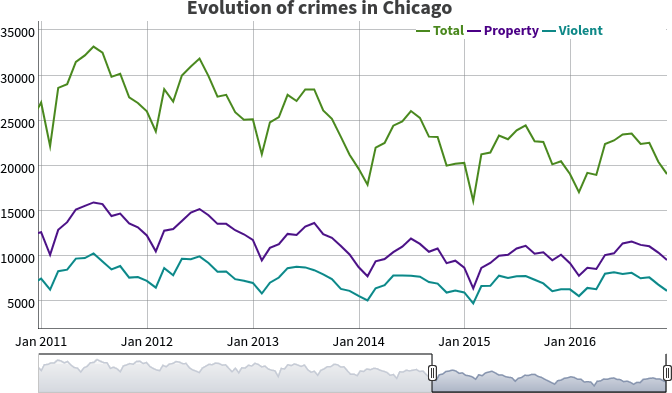
\includegraphics[width=0.8\textwidth]{images/single-chicago}
	\caption{Crime statistics in Chicago between January 2011 and December 2016}
	\label{fig:single-chicago}
\end{figure}

But this is just the analysis of one very specific city. Are more cities experiencing the same decrease in registered crimes? In figure \ref{fig:comp-base} we can see a comparison of four cities: Atlanta, Chicago, Philadelphia, and San Francisco (from the South, Midwest, Northeast, and West regions, respectively).

This time series opens a new picture on our understanding of crime statistics. It is well known that Chicago is particularly exemplary~\cite{Beardsley2014} on the early adoption of RMS systems, leading to an statistically robust data set. But how can we guess if this is the case with other cities? It is quite glaring that total crimes number by themselves are probably not the best number to analyse more than one city at the same time. For this reason we decided to give the user the ability to normalise data using two criteria: (a)~by population, depicted on figure \ref{fig:comp-pop}; and (b)~by crime mean\footnote{These ratios are widely used while comparing crime reports of different cities to study the relative time-evolution of crimes.~\cite{Boba2004}}.

\begin{figure}[H]
	\centering
	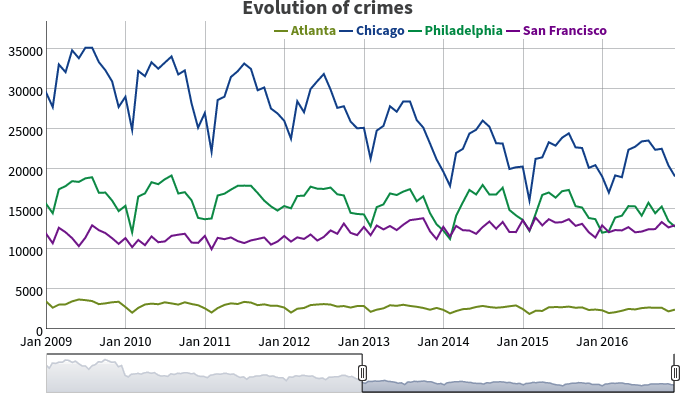
\includegraphics[width=0.8\textwidth]{images/base}
	\caption{Comparison of crime statistics between Atlanta, Chicago, Philadelphia, and San Francisco}
	\label{fig:comp-base}
\end{figure}

% \begin{figure}[H]
% 	\centering
% 	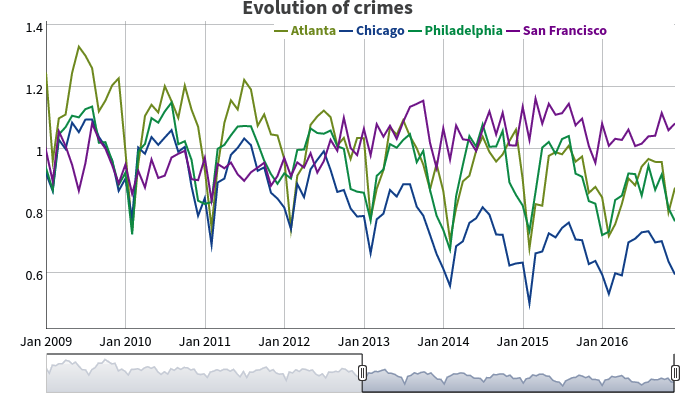
\includegraphics[width=0.8\textwidth]{images/mean}
% 	\caption{Comparison of crime statistics between Atlanta, Chicago, Philadelphia, and San Francisco; normalised by crime mean}
% 	\label{fig:comp-mean}
% \end{figure}

\begin{figure}[H]
	\centering
	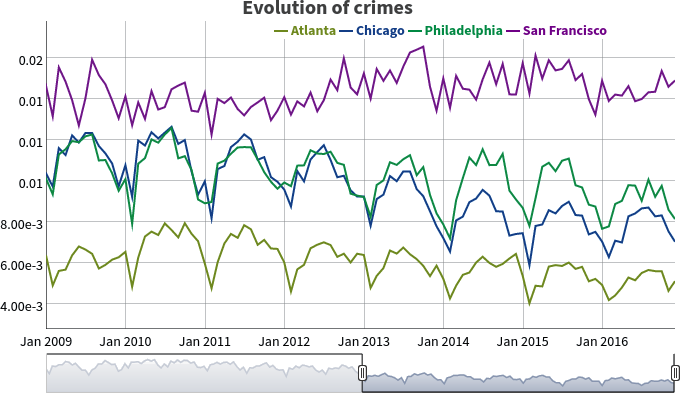
\includegraphics[width=0.8\textwidth]{images/pop}
	\caption{Comparison of crime statistics between Atlanta, Chicago, Philadelphia, and San Francisco; normalised by population}
	\label{fig:comp-pop}
\end{figure}

The differences in the three time series are remarkable. Using normalisation methods give us a much richer approach to do a qualitative comparative analysis. It is remarkable how different the West (San Francisco, Los Angeles, Portland, ...) is from the rest of the US: they are all seem to follow completely different cyclic patterns; crimes are on the rise, whilst the rest of the country seems to be improving their cities in regards to crime statistics.

Again, we could interpret these statistics in many ways. The obvious one seems to be that young and upper-class people, specially because of Hollywood and the Silicon Valley, are moving to the West coast, leading to more opportunities to commit crimes (usually property crimes). But without any proper analysis on the social predictors, this is just a wild conjecture. Quoting Rachel Boba~\cite{Boba2004},
\begin{quotation}
    \emph{All of these types of data serve a purpose in providing a picture of crime. However, depending on which data are used the picture may be very different.}
\end{quotation}


\bigskip
Last but not least, we would like to talk about Seattle (figure \ref{fig:single-seattle}). We included this city as an example of why data scientists and data analysts are required in today's world. When we first saw the data, we were quite shocked. How come there is such a huge gap of data between February 2013 and August 2014?

What we found is that for some reason, they don not have the \emph{Event Clearance Date} for most of the crimes reported in this period, but they do have the \emph{General Offense Number} (in the format \inline{YYYYN}, where \inline{YYYY} is the year \inline{N} seems to be an internal tracking code); this surely could be used by a data scientist to repopulate the missing values using data governance techniques.

\begin{figure}[H]
	\centering
	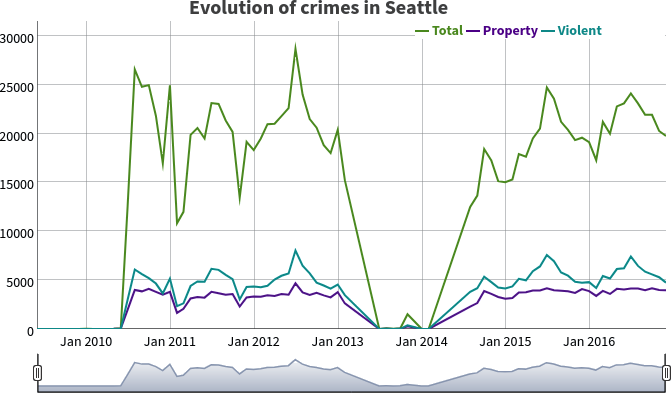
\includegraphics[width=0.8\textwidth]{images/single-seattle}
	\caption{Crime statistics in Seattle between January 2011 and December 2016}
	\label{fig:single-seattle}
\end{figure}

%-----------------------------------------------------------------
%	TEMA
%	!TEX root = ./../main.tex
%-----------------------------------------------------------------
\section{Conclusions}
% SHOULD INCLUDE:
% Limitations and future work
\lipsum[1-2]


% \begin{appendices}
% %-----------------------------------------------------------------
%	APPENDIX A
%	!TEX root = ./../main.tex
%-----------------------------------------------------------------
\section{Developed code}\label{app:code}
\renewcommand{\lstlistingname}{Script}
The code developed for this thesis is licensed under the \href{https://www.gnu.org/licenses/gpl-3.0.en.html}{GNU General Public License v3.0} and can be downloaded from \url{https://github.com/aldomann/tropical-cyclones}.

\lstinputlisting[firstline = 4, label = scr:hurdat2_base,%
	caption = \inline{hurdat2_base.R} - Base code to study the PDI of hurricane data from the National Hurricane Center (HURDAT)]%
	{code/hurdat2_base.R}
\lstinputlisting[firstline = 4, label = scr:hurdat2_pdi_base,%
	caption = \inline{hurdat2_pdi_base.R} - Base code to study the PDI probability density (DPDI)]%
	{code/hurdat2_pdi_base.R}
\lstinputlisting[firstline = 4, label = scr:hadisst_base,%
	caption = \inline{hadisst_base.R} - Base code to study the SST data from the Hadley Centre (HadISST)]%
	{code/hadisst_base.R}
\lstinputlisting[firstline = 4, label = scr:analysis_base,%
	caption = \inline{analysis_base.R} - Base code with several functions needed in \inline{main_analysis.R}]%
	{code/analysis_base.R}
\lstinputlisting[firstline = 4, label = scr:main_analysis,%
	caption = \inline{main_analysis.R} - Code to study the PDI dependence with the SST]%
	{code/main_analysis.R}
\lstinputlisting[firstline = 4, label = scr:hadcrut4_analysis,%
	caption = \inline{hadcrut4_analysis.R} - Code to study the global average temperature (from HadCRUT4)]%
	{code/hadcrut4_analysis.R}



% \end{appendices}

%-----------------------------------------------------------------
%	BIBLIOGRAPHY
%-----------------------------------------------------------------
% \nocite{Domingo2012}
\nocite{Beardsley2014}
\nocite{Wortley2008}
\nocite{McCue2015}
\nocite{Boba2004}
\nocite{ChicagoPoliceDepartment2017}

\printbibliography[heading=bibintoc]
% \setcounter{secnumdepth}{0}
% \section{References}
% \printbibliography[title={Articles}, type=article, heading=subbibliography]
% \printbibliography[title={Books}, type=book, heading=subbibliography]
% \printbibliography[title={Websites}, type=online , heading=subbibliography]
% \printbibliography[title={Other}, type=misc , heading=subbibliography]

\end{document}
